\documentclass{article}
\usepackage{graphicx} % Required for inserting images
\usepackage{amssymb} 
\usepackage{amsmath}
\usepackage{amsfonts}
\usepackage{relsize}
\usepackage{tikz-cd}
\usepackage{mathtools}
\usepackage{float}
\renewcommand{\oplus}{\mbox{\smaller$\bigoplus$}}
\renewcommand{\otimes}{\mbox{\smaller$\bigotimes$}}
\def\acts{\curvearrowright}

\title{MASA03 Lab 3}
\author{Isak Blom, Egor Jakimov, Simon Gustafsson}
\date{November 2025}

\begin{document}

\maketitle

\section*{Introduction to Estimators}
Let $X \sim F_\theta, \text{ } \theta \in \Theta$ and $x_1,\ldots, x_n$ independent observations of $X$. We wish to find a candidate for what $theta$ might be based on these observations. To this end, we construct what is called an \textit{estimator}. An estimator is simply a function $h:\mathbb{R}^n \to \Theta$. There are multiple commonly used estimators. For example: plug-in estimator, maximum-likelihood estimator and least-square estimator. 

\section{Confidence Intervals}

Suppose that $x_1,\dots,x_n$ are independent observations of $X\sim F_\theta$, where $\theta\in\Theta$ is a parameter on which the distribution function depends. Let $\hat{\theta}=h(x_1,\dots,x_n)$ be an estimator of $\theta$ (e.g. the plug-in estimator). Then we can view $\hat{\theta}$ as a random variable by setting $\hat{\theta} = h(X_1,\dots,X_n)$ where $X_k\sim F_\theta$. Then, if $I\subseteq\Theta$ is such that $\mathbb{P}(\hat{\theta}\in I)=1-\alpha$, we say that $I$ is a confidence region with level $1-\alpha$ (if $\Theta\subseteq\mathbb{R}$ and $I$ is an interval, it is called a confidence interval).\\

\section{Hypothesis Testing}
Suppose that $x_1,\ldots,x_n$ are independent observations of $X \sim F_\varphi$ where $\varphi \in \Theta$. Form hypotheses \[\begin{cases} H_0: \varphi \in A\\ H_1: \varphi \notin A\end{cases},\]
 \textit{statistic} $T: \mathbb{R}^n \to \mathbb{R}$, \textit{critical region} $C \subseteq \mathbb{R}$, and reject our hypothesis $H_0$ if $T(x_1,\ldots,x_n) \in C$. In order to define $T$ and $C$ define the power function \[\pi(\theta)=\mathbb{P}\left(T\left(X_{\theta}^{(1)},\dots,X_{\theta}^{(n)}\right)\in C\right)\] where $X_{\theta}^{(i)}\sim F_{\theta}$. We want to choose the function $T$ and the critical region $C$ such that $\alpha \coloneq\sup_{\theta \in A}\pi(\theta)$ is small and for any $\theta \notin A$ we have $\pi(\theta) > \alpha$. This construction will give that if our data was distributed as $F_{\theta}$ with $\theta\in A$, it is unlikely that our hypothesis is rejected, and if $\theta \notin A$ it is more likely that our hypothesis is rejected. Ideally we want $\pi(\theta)$ to be much bigger than $\alpha$ for $\theta \notin A$. \\
 In the case that $A=\{\theta_0\}$ (i.e. $A$ is a singleton), the corresponding $H_0$ is then called a \textit{simple} null hypothesis, and the supremum in the definition of $\alpha$ is just $\pi(\theta_0)$.

\section{Exercises}
\subsection{1.}

\begin{figure}[H]
    \centering
    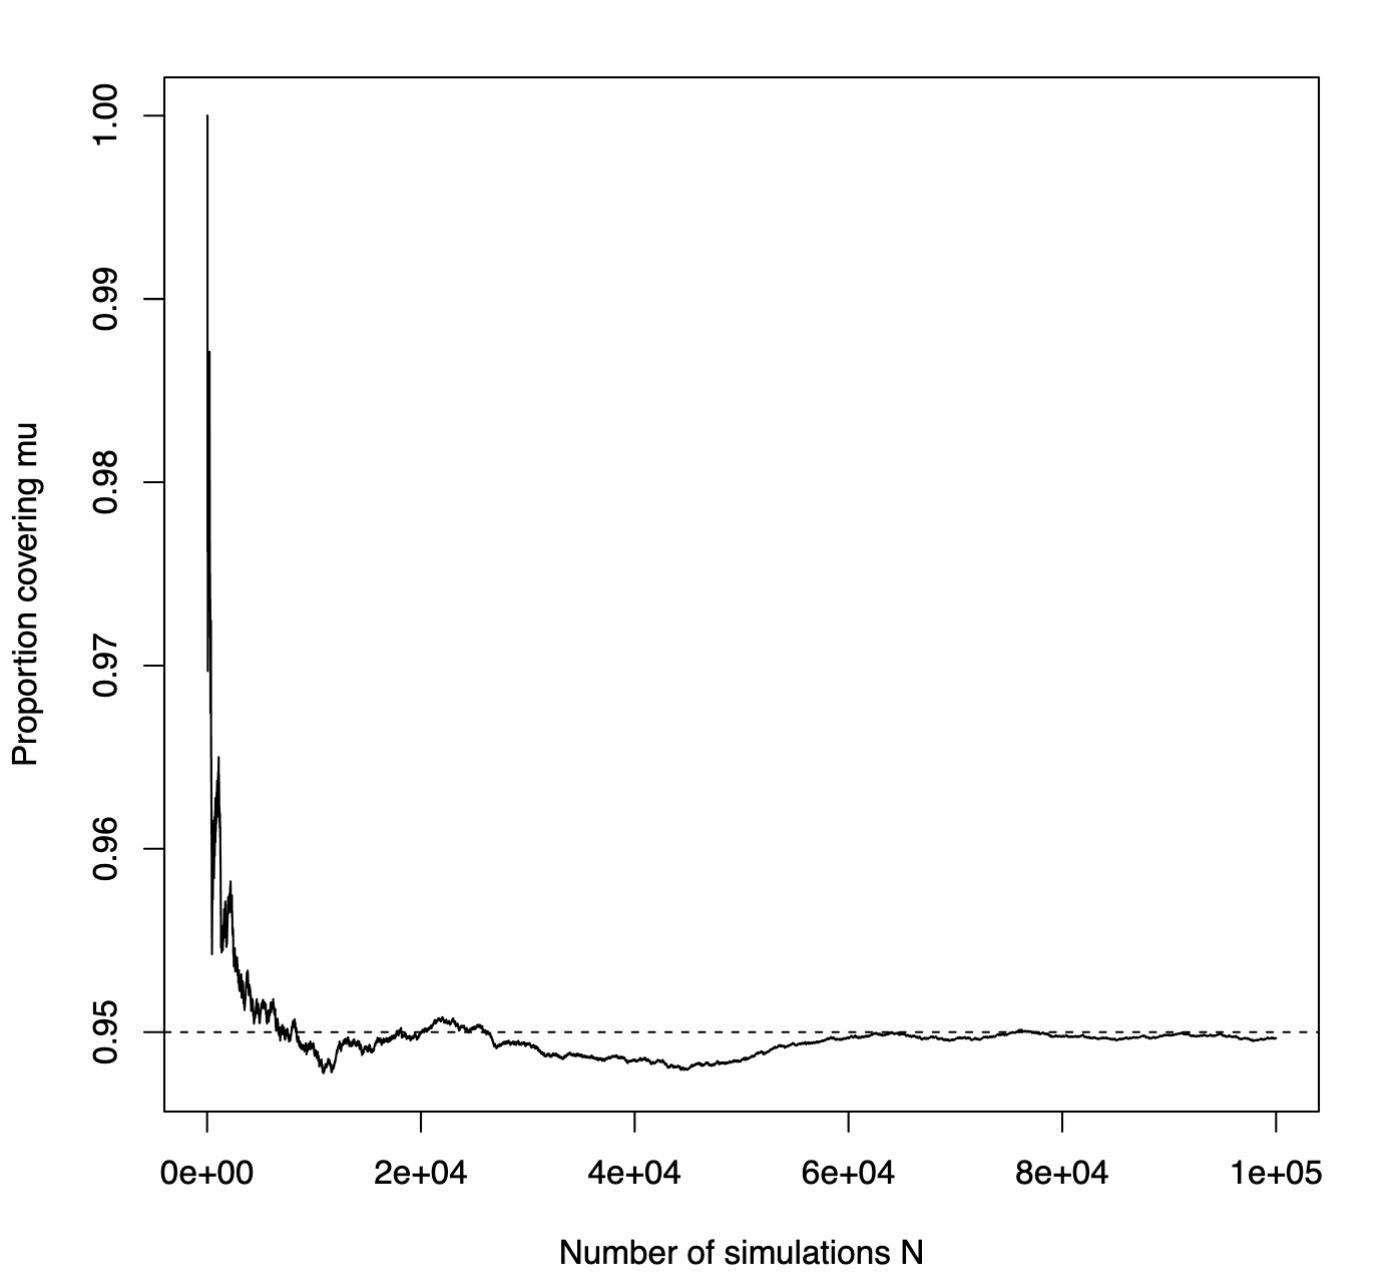
\includegraphics[width=0.75\linewidth]{figures/Exercise 1 (2).png}
        \caption{Exercise 1}
    \label{fig:placeholder}
\end{figure}

\subsubsection{(a)} 
The simulated covering proportion is close to $0.95$, and the running coverage plot stabilizes near $0.95$, so the theoretical value appears correct.

\subsubsection{(b)}
\[
I_i = \mathbf{1}\{\mu \text{ lies inside the } i\text{th simulated confidence interval}\},
\] 
The variables $I_1,\dots,I_N$ are i.i.d.\ Bernoulli$(0.95)$.  
By the Law of Large Numbers,
\[
\frac{1}{N}\sum_{i=1}^N I_i \longrightarrow 0.95
\quad \text{as } N \to \infty.
\]
Hence the measured proportion of intervals containing $\mu$ converges to the true coverage probability $0.95$.
\subsection{2.}
\begin{figure}[H]
        \centering
        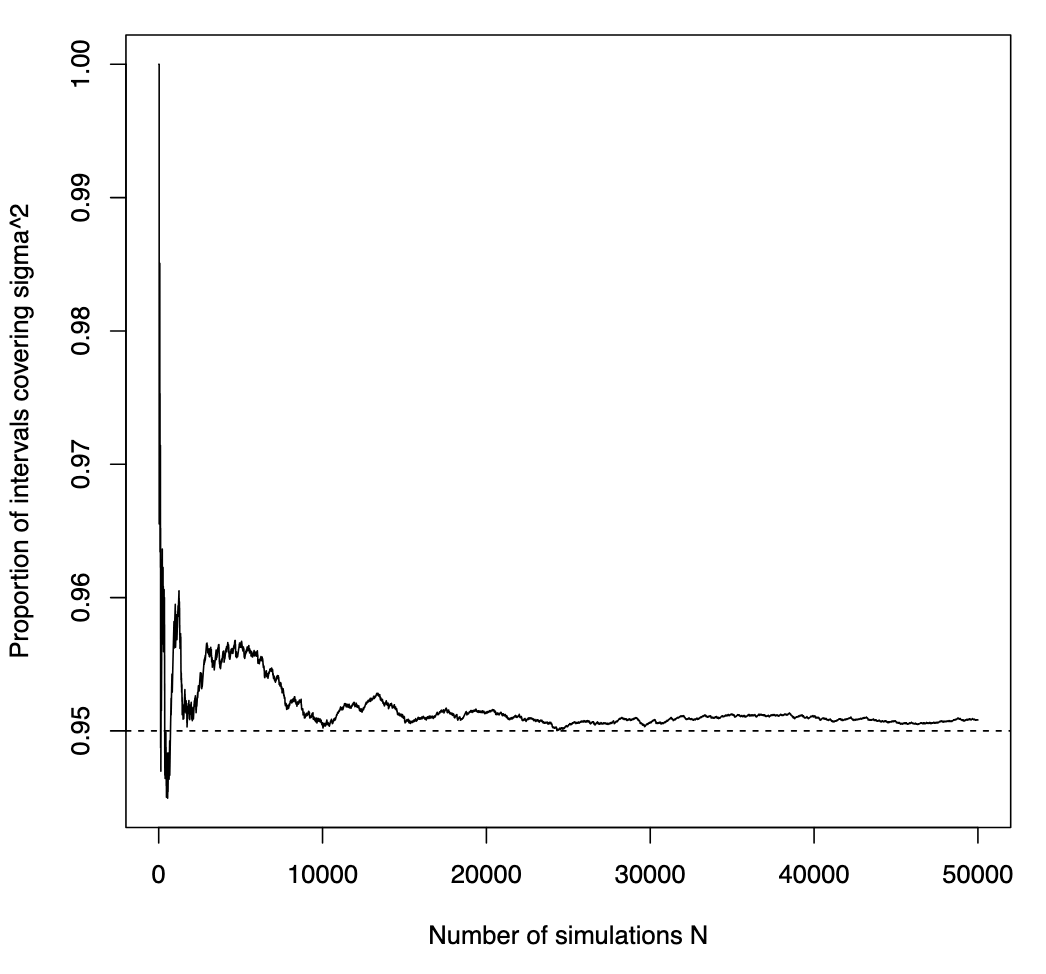
\includegraphics[width=0.75\linewidth]{figures/Exercise 2.png}
        \caption{Exercise 2}
        \label{fig:placeholder}
    \end{figure}

\subsubsection{(a)} 
The simulated covering proportion is close to $0.95$, and the running coverage plot stabilizes near $0.95$, so the theoretical value appears correct.

\subsubsection{(b)} 
\[
I_i = \mathbf{1}\{\sigma^2 \text{ lies inside the } i\text{th simulated confidence interval}\}.
\]
The variables $I_1,\dots,I_N$ are i.i.d.\ Bernoulli with mean $0.95$.  
By the Law of Large Numbers,
\[
\frac{1}{N}\sum_{i=1}^N I_i \longrightarrow 0.95
\quad\text{as } N \to \infty.
\]
Hence the empirical proportion of intervals covering $\sigma^2$ converges to the true coverage probability $0.95$.

\subsection{3.}

\subsubsection{(a)} 
The simulated rejection proportion is close to $0.05$, so the test attains the intended significance level.

\subsubsection{(b)} 
Let $I_i$ denote the indicator that the $i$th simulated test rejects $H_0$.  
The variables $I_1,\dots,I_N$ are i.i.d.\ Bernoulli with mean $0.05$.  
By the Law of Large Numbers,
\[
\frac{1}{N}\sum_{i=1}^N I_i \longrightarrow 0.05
\quad \text{as } N \to \infty.
\]
Thus the empirical rejection proportion converges to the true significance level.


\subsection{4}
\begin{figure}[H]
    \centering
    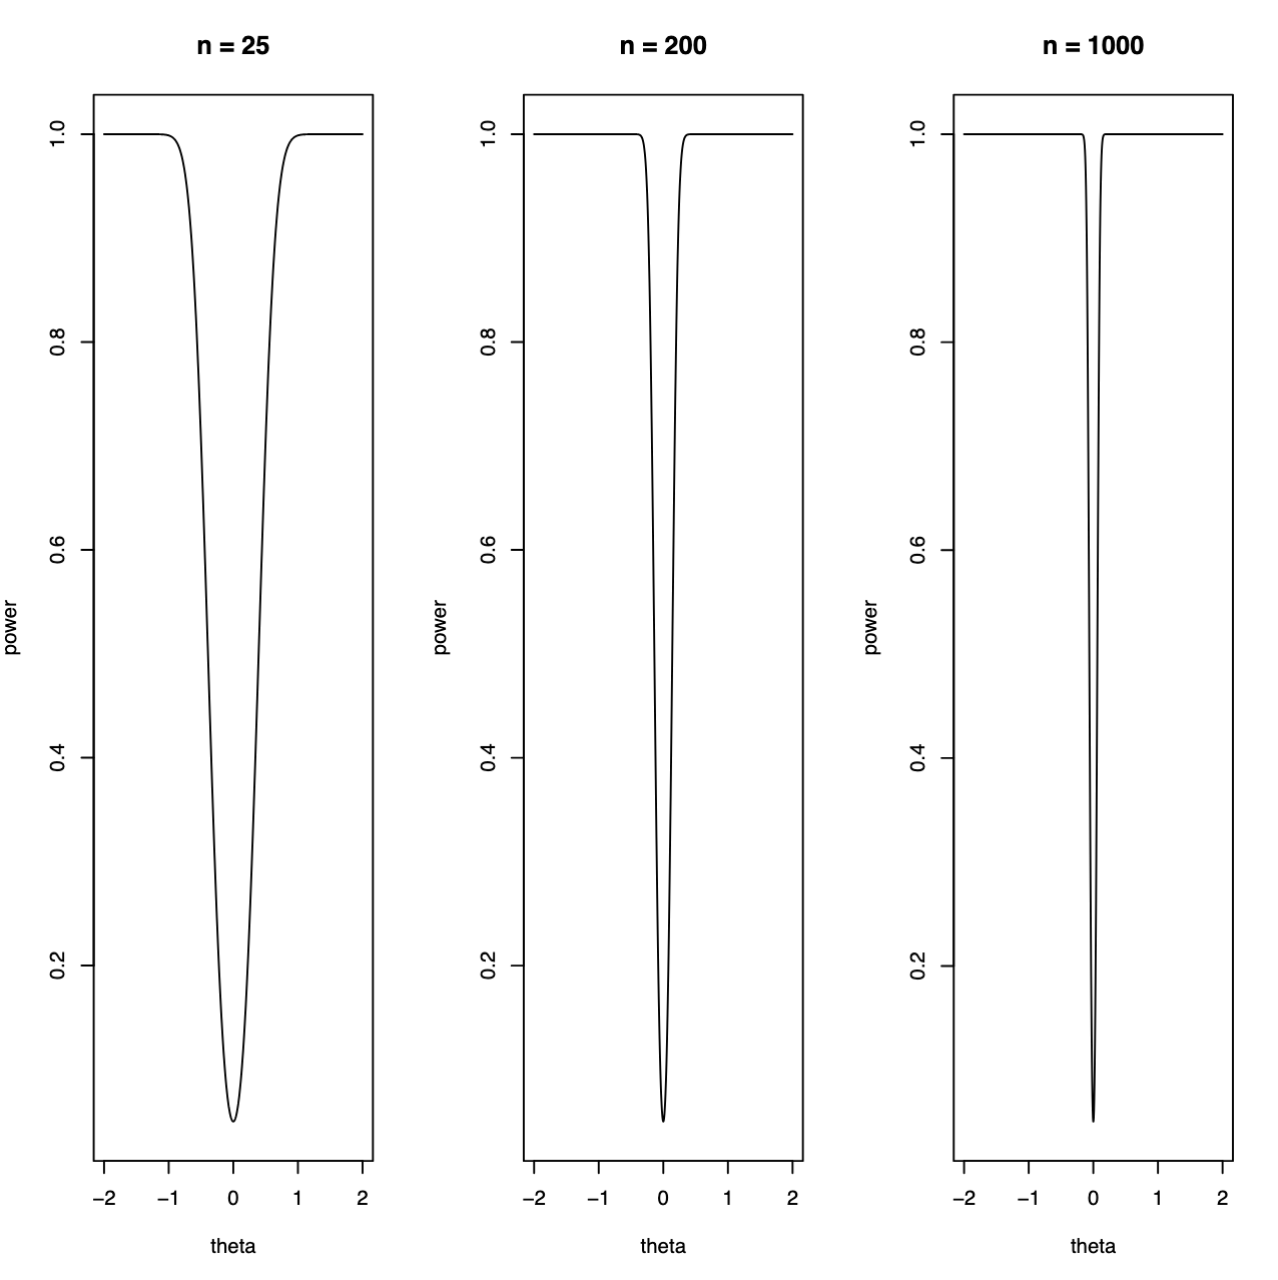
\includegraphics[width=0.75\linewidth]{figures/Exercise 3.png}
    \caption{Enter Caption}
    \label{fig:placeholder}
\end{figure}

\subsubsection{(a)}
When $n = 200$, the power curve has the expected shape: it stays near $0.05$ at $\theta = 0$, and then rises as $\theta$ moves away from $0$. The test rarely rejects when the null is true, and it becomes increasingly likely to reject when the true mean differs from $0$.

\subsubsection{(b)}
With only $n = 25$ points, the power curve is much flatter. The test has noticeably less ability to detect nonzero values of $\theta$. In other words, smaller samples make it harder for the test to distinguish between $H_0$ and $H_1$.

\subsubsection{(c)}
For $n = 1000$, the power curve becomes very steep. Even small changes in $\theta$ away from $0$ lead to power close to $1$. This happens because with a very large sample, the test can detect even tiny deviations from the null hypothesis.


\end{document}
